% This is auto-generated file: do not edit!
% Exported from microMathematics Plus, version 2.17.2


Данный пример демонстрирует
вычисление степенных рядов и
интегралов.

\subsection{Ряд Тейлора}

Рядом Тейлора является разложение
функции в бесконечный степенной
ряд, коэффициенты которого
вычисляются с использованием
производных исходной функции.

Например, разложение в ряд Тейлора
функции в окрестности точки x, где
количество членов степенного ряда
равно N, обозначим как Ts(x,N):
\begin{center}\begin{tabular}{c}
  $Ts(x,N) := \displaystyle\sum_{n=0}^{N} \frac{{ \left( -1\right) }^{n}}{\left( 2 \cdot n \right)! } \cdot {x}^{2 \cdot n}$
\end{tabular}\end{center}

Данное разложение аппроксимирует
функцию косинуса:
\begin{center}\begin{tabular}{c}
  $s(x) := cos \left( x\right) $
\end{tabular}\end{center}

Построим график обеих функций для
одного и того же интервала. На
первый взгляд, обе кривые
идентичны:
\begin{center}\begin{tabular}{c}
  $x := \left[ 0,\, 0.1 \,..\, 2 \cdot {\pi} \right]$
\end{tabular}\end{center}
\begin{center}\begin{tabular}{c} 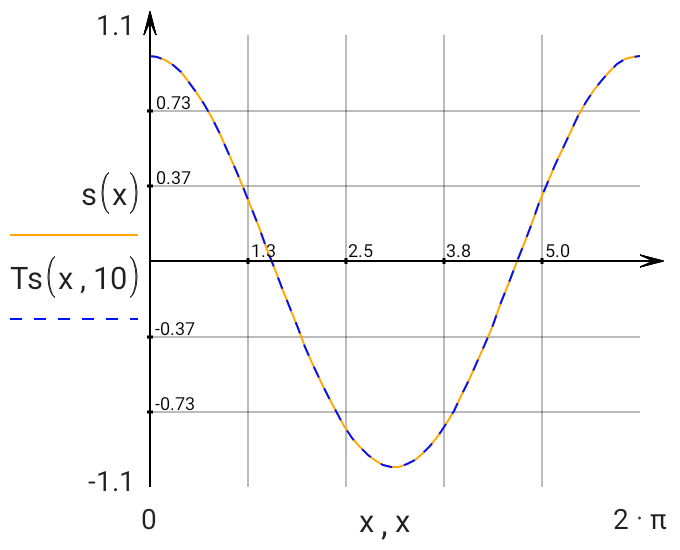
\includegraphics[resolution=320]{graphics/series_and_integrals_fig1.png} \end{tabular}\end{center}

На самом же деле, сумма ряда
Ts(x,N) вычислена с погрешностью,
которая обусловлена конечным
количеством членов ряда N. Введём
функцию невязки $\Delta$(x,N), которая
описывает эту погрешность:
\begin{center}\begin{tabular}{c}
  ${\Delta}(x,N) :=  \left| s \left( x\right)  - Ts \left( x,\, N\right)  \right| $
\end{tabular}\end{center}

Построим график этой функции в
зависимости от количества членов
ряда. В данном случае, удобнее
использовать логарифмическую ось
ординат. Тогда мы увидим, что
порядок погрешности линейно
уменьшается с увеличением
количества членов ряда:
\begin{center}\begin{tabular}{c}
  $N := \left[ 3,\, 4 \,..\, 13 \right]$
\end{tabular}\end{center}
\begin{center}\begin{tabular}{c} 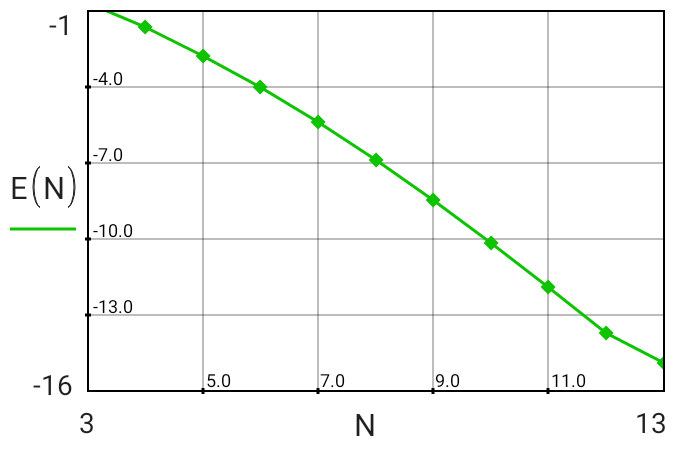
\includegraphics[resolution=320]{graphics/series_and_integrals_fig2.png} \end{tabular}\end{center}

\subsection{Биномиальный ряд}

Рассмотрим степенную функцию
\begin{center}\begin{tabular}{c}
  $f(x,{\alpha}) := {\left( 1 + x \right)}^{{\alpha}}$
\end{tabular}\end{center}

Эту функцию можно разложить в
биномиальный ряд:
\begin{center}\begin{tabular}{c}
  $Tf(x,{\alpha},N) := \displaystyle\sum_{n=0}^{N}  \left( \displaystyle\prod_{k=1}^{n} \frac{{\alpha} - k + 1}{k}\right)  \cdot {x}^{n}$
\end{tabular}\end{center}

Также как и в предыдущем примере,
можно построить графики обеих
функций. Несмотря на то, что
исходная и аппроксимированная
функции визуально совпадают, здесь
также имеется погрешность,
связанная с конечным числом членов
ряда:
\begin{center}\begin{tabular}{c} 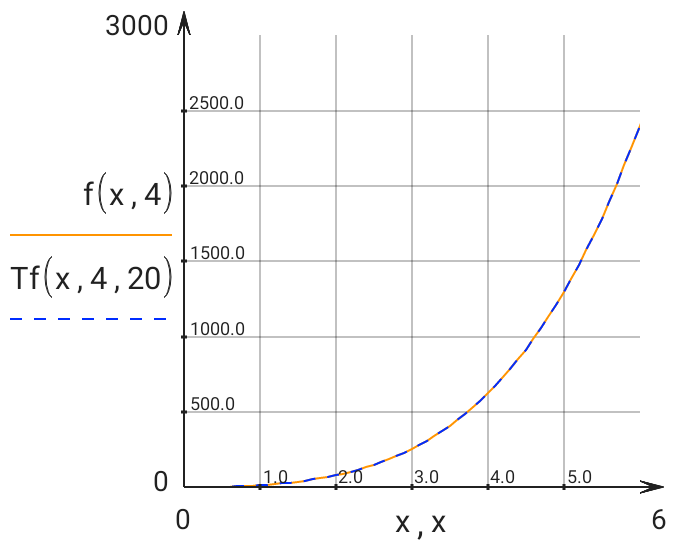
\includegraphics[resolution=320]{graphics/series_and_integrals_fig3.png} \end{tabular}\end{center}

\subsection{Интегралы}

Программа также предоставляет
возможность вычисления
определённых интегралов методом
Симпсона. К примеру, можно
вычислять интегралы с
использованием элемента ''Текстовый
результат'':
\begin{center}\begin{tabular}{c}
  $\displaystyle\int_{0}^{3 \cdot pi / 2}{cos \left( \frac{2 \cdot x}{9}\right) }^{-2}\, dx = 7.79423$
\end{tabular}\end{center}

Аналитическое решение для данного
интеграла выглядит следующим
образом:
\begin{center}\begin{tabular}{ccc}
  $I := \frac{9 \cdot \sqrt{3} }{2}$ &
  ,    &
  $I = 7.79423$ \cr
\end{tabular}\end{center}

Так как интеграл найден не
аналитически, а с использованием
численного метода, то имеет место
быть следующая погрешность:
\begin{center}\begin{tabular}{c}
  $\displaystyle\int_{0}^{3 \cdot pi / 2}{cos \left( \frac{2 \cdot x}{9}\right) }^{-2}\, dx - I = 4.26681E-9$
\end{tabular}\end{center}

Эта погрешность зависит от
параметра ''Значимые цифры в
результате''. Данный параметр
задаётся в окне ''Свойства
документа'', которое вызывается из
верхней панели инструментов:
\begin{center}\begin{tabular}{c} 
\includegraphics[resolution=320]{graphics/series_and_integrals_fig4.png} \end{tabular}\end{center}

При увеличении этого параметра,
точность вычисления интеграла
увеличивается, но увеличивается
также и время, необходимое для его
вычисления.